\def\directorynameimg{./include/img}
\chapter{Sistema de Gestão de Incidentes}
\section{Introdução}
O sistema de gestão de incidentes (SGI) é uma ferramenta que permite criar e consultar pedidos ao Departamento de Operações e Suporte da Eurotux.
%Permite obter respostas a pedidos de informações e de \textit{help desk} de forma eficiente.
Sublinha-se que a sua utilização é essencial para garantir uma resposta rápida e o melhor acompanhamento dos incidentes reportados. 

O SGI está acessível através de uma interface \textit{web} no seguinte endereço:
\begin{itemize}
	\item \url{https://suporte.eurotux.com}
\end{itemize}

\section{Contactos}\label{sgi:contactos}
O Departamento de Operações e Suporte da Eurotux pode ser contactado pelos seguintes meios:
\begin{itemize}
\item Telefone: +351 253 680 301 (Portugal) ou +258 848 777 419 (Moçambique).
\item \textit{Email} de suporte personalizado (indicado pela Eurotux), cujo formato é \\ \texttt{<empresa>@suporte.eurotux.com}.
\item \textit{Email} geral do Departamento de Operações e Suporte: \texttt{suporte@eurotux.com}.
\end{itemize}

\section{Observações}
Quaisquer dúvidas ou informações adicionais relativamente à utilização da ferramenta devem ser enviadas para o \emph{email} \texttt{suporte@eurotux.com}.

É importante que sejam efetuados testes de utilização logo que possível. Sugere-se a criação/abertura de um \emph{\textit{ticket}} com o \emph{Assunto/\textit{Subject}} ``teste'' para experimentar as funcionalidades descritas neste manual. Deste modo, será possível efetuar uma aprendizagem progressiva no uso da ferramenta.

\chapter{Instruções de Utilização}
\section{Introdução}
O funcionamento das funções mais utilizadas do SGI é descrito nesta secção de uma forma resumida, de modo a poder ser utilizado de imediato.

São descritas as seguintes operações:
\begin{itemize}
\item Acesso ao SGI.
\item Autenticação. 
\item Página inicial.
\item Criar \textit{ticket}.
\item Fechar \textit{ticket}.
\item Escalar \textit{ticket}/Reclamar.
\item Pesquisar \textit{tickets}.
\item Alterar definições do utilizador (\textit{password}, língua, etc.).
\item Sair.
\end{itemize}

\section{Aceder ao SGI}
Para se aceder à interface do SGI, deve abrir-se o seguinte endereço URL num \textit{browser}/navegador de Internet (Firefox, Chrome, Opera, Internet Explorer, Edge ou outro):

\begin{itemize}
\item \url{https://suporte.eurotux.com}
\end{itemize}

O acesso é efetuado através de uma ligação segura e encriptada\footnote{Ligação HTTPS. É identificada por um símbolo de um cadeado ou por uma referência a \textit{website} seguro (dependendo do \textit{browser} utilizado).}, assegurando a proteção do acesso e das operações efetuadas.

\section{Autenticação}
Ao aceder-se à página inicial do SGI (figura \ref{fig:rt1}), são pedidas as credenciais de acesso.
%, compostas por um nome de utilizador/\textit{username} e uma palavra-passe/\textit{password}. 
Estas credenciais são disponibilizadas pelo Departamento de Operações e Suporte da Eurotux.
Se não possuir as credenciais de acesso, por favor, contacte o Departamento de Operações e Suporte da Eurotux através dos meios referidos na secção \ref{sgi:contactos}.

%\begin{figure}[H]
%\begin{center}
%%\includegraphics[scale=0.45]{include/img/rt1}
%%\includegraphics[width=16cm,height=10.5cm]{include/img/rt1_1}
%\includegraphics[width=16cm]{include/img/rt1_1}
%\end{center}
%\caption{Página de Autenticação}
%\label{fig:rt1}
%\end{figure}

\begin{figure}[H]
\begin{center}
%\includegraphics[scale=0.45]{include/img/rt1}
%\includegraphics[width=16cm,height=10.5cm]{include/img/rt1_1}
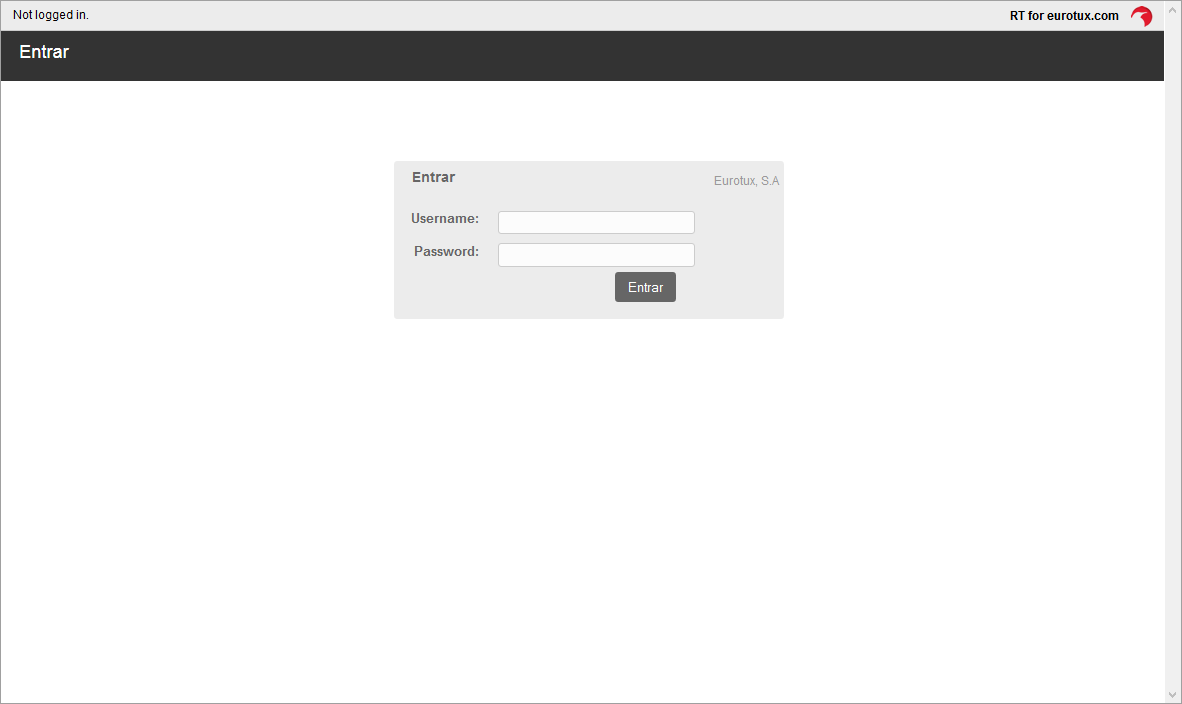
\includegraphics[width=16cm]{\directorynameimg/rt1-1}
\end{center}
\caption{Página de autenticação.}
\label{fig:rt1}
\end{figure}

\section{Página inicial}
Após se autenticar no SGI, é-se encaminhado para a página inicial (figura \ref{fig:rt2}) onde se efetua a gestão dos pedidos/incidentes.

\begin{figure}[H]
\begin{center}
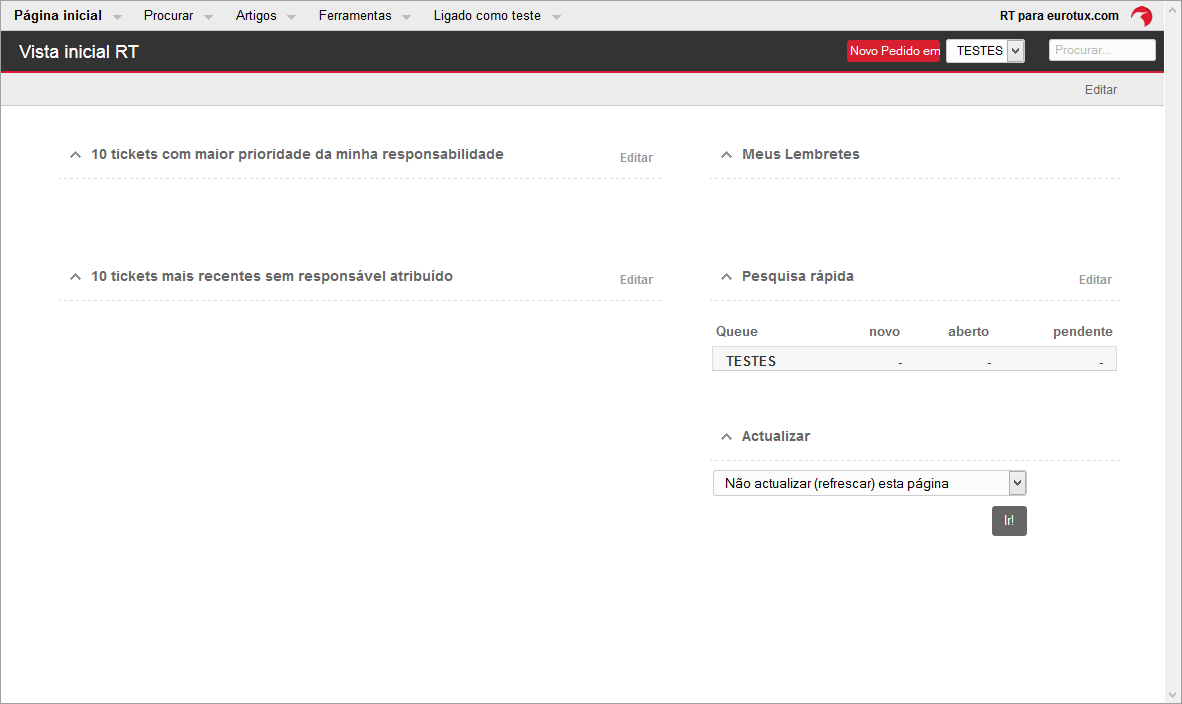
\includegraphics[width=16cm]{\directorynameimg/rt2-1-PT}
\end{center}
\caption{Página inicial.}
\label{fig:rt2}
\end{figure}

A página inicial possui agrupadores que apresentam os pedidos em aberto de forma organizada:

\begin{itemize}
\item \textbf{\textit{Tickets} com maior prioridade da minha responsabilidade} \\
Neste campo são apresentados os \textit{tickets} de incidentes abertos que são da responsabilidade do utilizador.
É possível definir o número de \textit{tickets} a visualizar neste campo e o seu modo de ordenação.

\item \textbf{\textit{Tickets} mais recentes sem responsável atribuído} \\
Neste campo são apresentados os \textit{tickets} de incidentes abertos que se encontram a aguardar pela atribuição de um técnico responsável pela resolução.
É possível definir o número de \textit{tickets} a visualizar neste campo e o seu modo de ordenação.

\item \textbf{Meus Lembretes} \\
Neste campo é possível visualizar as notificações (ou lembretes) existentes, relativos a alguma ação associada a um \textit{ticket}. Por exemplo, efetuar um contacto, fazer um ponto de situação, etc.

\item \textbf{Pesquisa rápida} \\
No ecrã que aparece imediatamente após a autenticação, existe uma coluna no lado direito identificada como \emph{Pesquisa rápida/\textit{Quick Search}} em que existe um único item (\emph{queue}).
É nessa \emph{queue} que estarão os pedidos de suporte/\textit{help desk} (\emph{tickets}) ainda abertos (\textit{open}).

\item \textbf{Atualizar}
Nesta caixa de seleção, é possível definir a frequência de atualização da informação disponibilizada na página inicial.
\end{itemize}


%\begin{figure}[H]
%\begin{center}
%\includegraphics[width=15cm]{include/img/rt2_1}
%\end{center}
%\caption{Página Inicial}
%\label{fig:rt2}
%\end{figure}

\section{Criar \textit{ticket}}
Para se criar um novo \textit{ticket}, seleciona-se \emph{Novo \textit{ticket}} em \emph{New Ticket In}. De seguida, seguem-se os seguintes passos:
\begin{itemize}
	\item Preencher o campo \emph{Assunto/\textit{Subject}} com o assunto relativo ao \textit{ticket}.
	\item Preencher o campo \emph{Descreva o pedido, abaixo/\textit{Describe the issue below}} (ver figura \ref{fig:rt3}) com a descrição do incidente. Deve apresentar-se toda a informação disponível que possa auxiliar na resolução do mesmo;
	\item Após se preencher a descrição do incidente, clicar no botão \emph{Criar/\textit{Create}} que se situa do lado direito, abaixo da caixa de texto da descrição do incidente;
	\item O incidente fica registado e acessível aos técnicos da Eurotux, que irão aceder à informação registada e dar o devido seguimento.
\end{itemize}

\bigskip

\textbf{Campos de preenchimento opcional:}
\begin{itemize}
\item \textbf{Cc} \\
Se desejado, podem adicionar-se outros endereços de \textit{email} neste campo, o que permitirá que as interações no SGI sejam enviadas aos mesmos. Esta funcionalidade permite que utilizadores não registados %na \textit{comunidade de utilizadores} 
visualizem as interações ocorridas num \emph{ticket}.
\item \emph{\textbf{Anexar ficheiro/Attach file:}}
Podem anexar-se ficheiros ao \emph{ticket} para complementar a informação sobre o incidente, ou para registo.
\end{itemize}

\bigskip

Os utilizadores que têm acesso a uma \textit{queue} recebem sempre, por \textit{email}, o conteúdo colocado nessa \emph{queue} pelos outros utilizadores. A lista de utilizadores é normalmente constituída pelos endereços de \textit{email} do cliente (um ou mais) e dos técnicos da Eurotux.

Após a receção do \textit{email}, é possível interagir com o SGI a partir desse meio. Para tal, basta responder de forma habitual, mantendo a identificação do \textit{ticket} no assunto\footnote{Exemplo: [eurotux.com \#000000] \ldots }. A mensagem contida no corpo do \textit{email} de resposta será adicionada ao \textit{ticket} em causa, ficando disponível na interface \textit{web}. 

\textbf{Nota:} O SGI só regista mensagens enviadas a partir de endereços de \textit{email} que fazem parte da lista de utilizadores. 

Nas respostas, deve retirar-se o máximo de informação não relevante e apenas colocar o que é informação nova. A ferramenta, por si, já constitui um histórico das diversas interações.


\begin{figure}[H]
\begin{center}
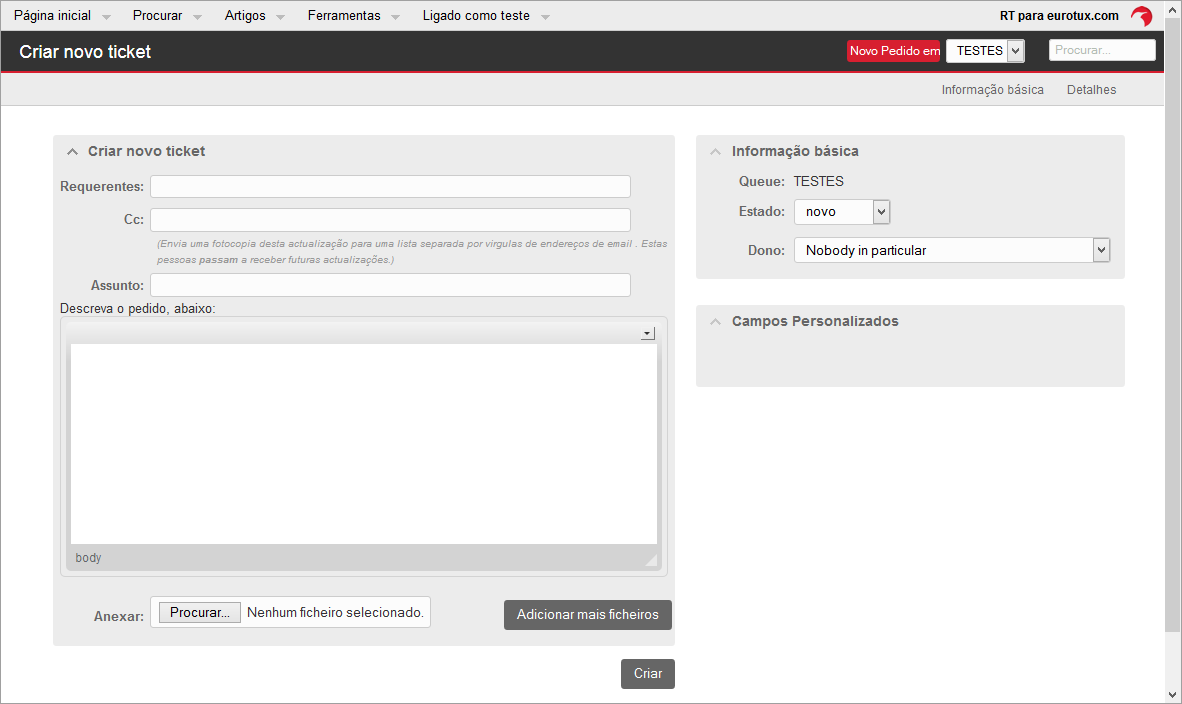
\includegraphics[width=16cm]{include/img/rt3-1-PT}
\end{center}
\caption{Criar \textit{ticket}.}
\label{fig:rt3}
\end{figure}

\section{Fecho de \emph{tickets}}
Os \textit{tickets} devem ser encerrados pelo cliente. O seu encerramento constitui uma forma de aprovação e validação das atividades desenvolvidas, significando que o assunto/intervenção está concluído.

Para se encerrar um \emph{ticket}, seleciona-se a opção \emph{Resolver/\textit{Resolve}} que aparece no menu \emph{Acções/\textit{Actions}} no canto superior direito do ecrã onde se está a visualizar um determinado \emph{ticket} (ver figura \ref{fig:rt6}).

Opcionalmente, é possível efetuar nova entrada de texto ao fechar um \textit{ticket}. Pode ser, por exemplo, a confirmação de que os trabalhos foram efetuados com sucesso e que o incidente se encontra resolvido, ou qualquer outra informação relevante.

Os \textit{tickets} não aparecem na visualização por omissão depois de encerrados.

\begin{figure}[H]
\begin{center}
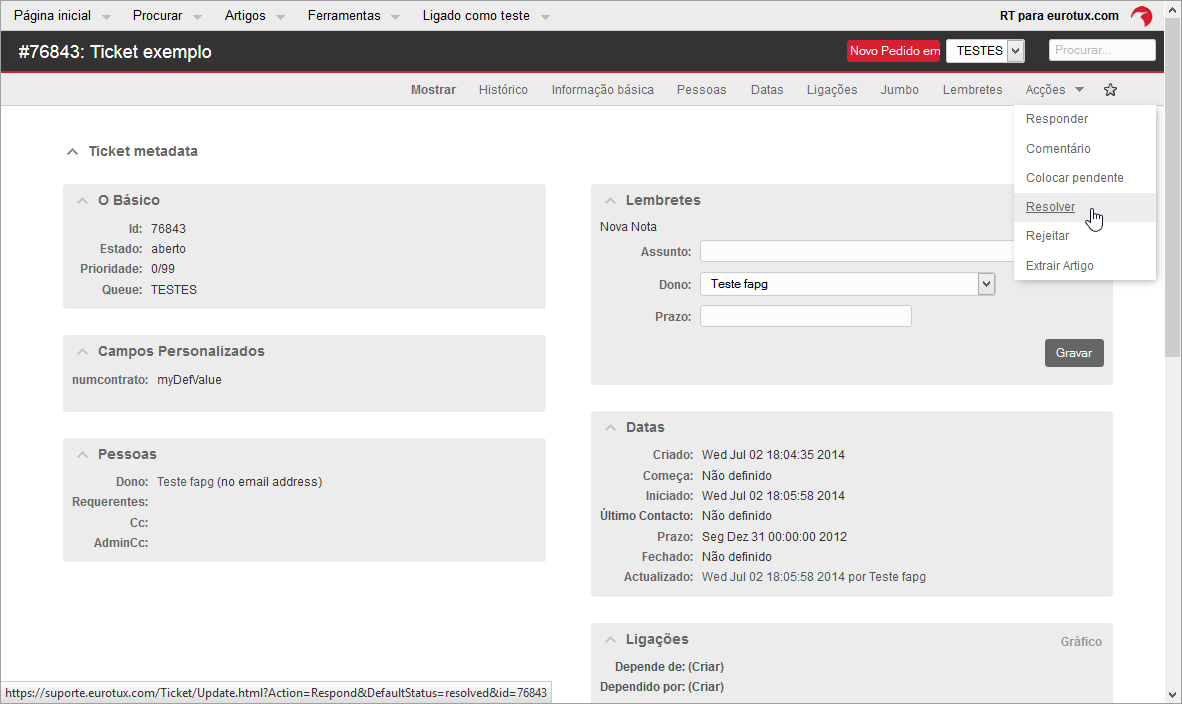
\includegraphics[width=16cm]{\directorynameimg/rt6-1-PT}
\end{center}
\caption{Fechar \textit{ticket}.}
\label{fig:rt6}
\end{figure}

\section{Escalar \textit{ticket}/Reclamar} 
O SGI disponibiliza uma opção, denominada \emph{Reclamar}, que permite ao cliente reportar a situação quando considerar que a resposta ao \textit{ticket} em questão não está a ser adequada.

Para registar uma reclamação, preenche-se o campo \emph{Reclamar} (ver figura \ref{fig:rt7}), fornecendo a descrição dos factos relevantes. De seguida, clica-se no botão \emph{Enviar} que se encontra junto à caixa de texto.

A reclamação será registada e transmitida aos responsáveis do Departamento de Operações e Suporte e do Departamento de Qualidade, que efetuarão a análise e darão diligência aos procedimentos adequados.

\begin{figure}[H]
\begin{center}
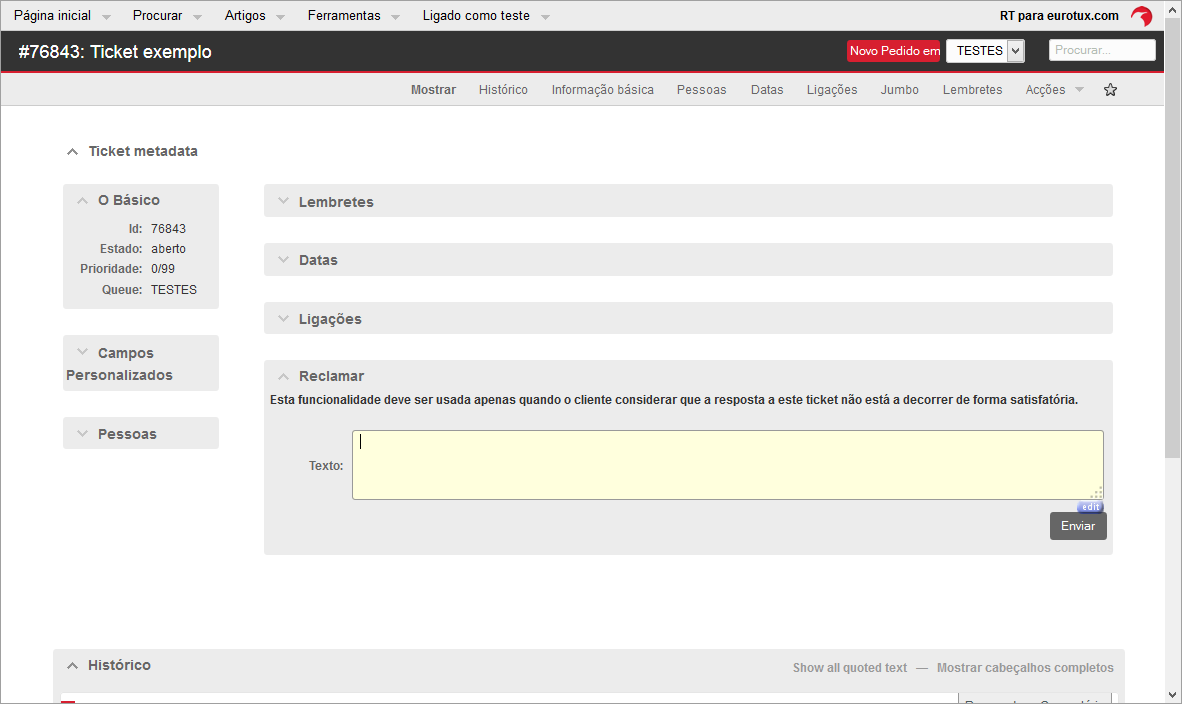
\includegraphics[width=16cm]{\directorynameimg/rt7-1-PT}
\end{center}
\caption{Escalar \textit{ticket}/Reclamar.}
\label{fig:rt7}
\end{figure}


\section{Pesquisar \textit{tickets}}
O SGI permite fazer pesquisas simples, por número do \textit{ticket} ou por parte do seu assunto, por exemplo, ou mais avançadas.

Para pesquisar, acede-se a \textbf{\emph{Procurar/\textit{Search}} > \emph{\textit{Tickets}} > \emph{Nova Pesquisa/\textit{New Search}}} (ver figura \ref{fig:rt4}). De seguida, preenchem-se os campos adequados para obter os \emph{tickets} que obedeçam aos critérios definidos.

Sabendo o número de um \textit{ticket}, é possível aceder diretamente ao mesmo. 
Para isso, utiliza-se caixa \emph{\textit{Search}} localizada no lado direito do ecrã, na parte superior.

\begin{figure}[H]
\begin{center}
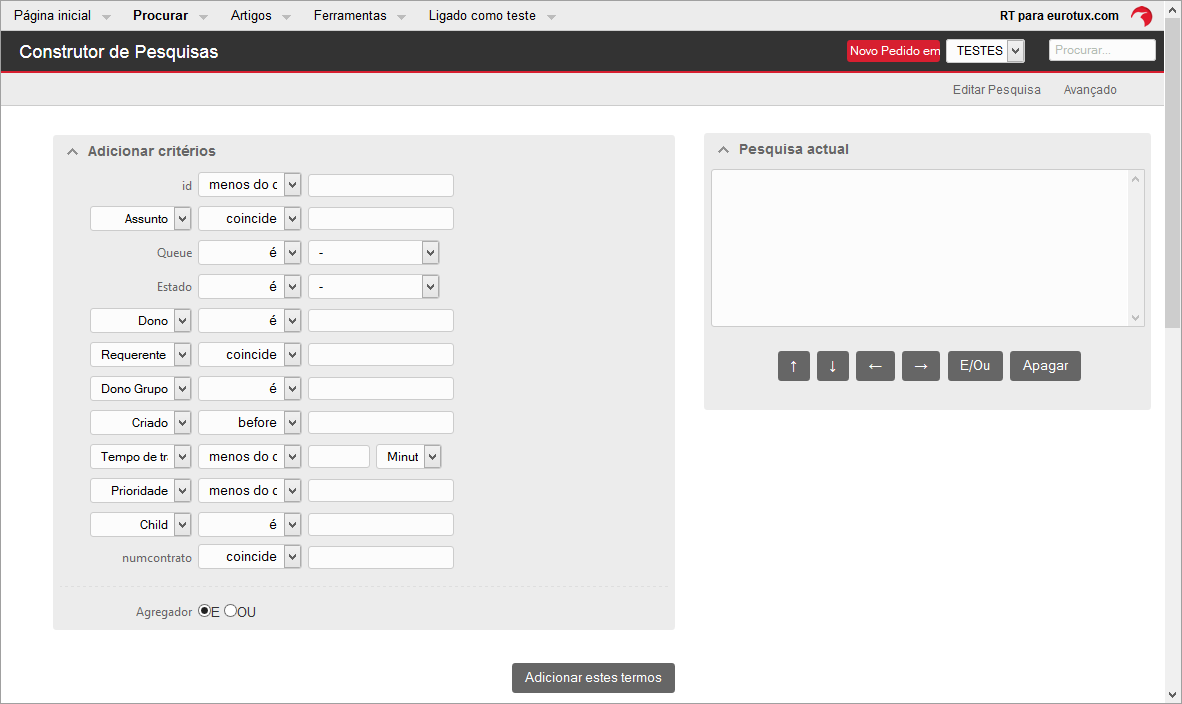
\includegraphics[width=16cm,height=9cm]{include/img/rt4-1-PT}
\end{center}
\caption{Procurar \textit{tickets}.}
\label{fig:rt4}
\end{figure}

\section{Preferências}
Recomenda-se a alteração da \textit{password} indicada pelo Departamento de Operações e Suporte por uma à escolha do utilizador.

Para se alterar \textit{password}, acede-se a \textbf{\emph{Ligado como.../\textit{Logged in as...}} > \emph{Configurações/\textit{Settings}} > \emph{Acerca/\textit{About}}} (ver figura \ref{fig:boot}). A \textit{password} de acesso ao SGI, o idioma e outros dados acerca do utilizador podem ser alterados neste painel.

Também se recomenda que, na seleção do idioma para Português, seja utilizado a opção \textbf{\textit{Portuguese}} em vez das opções \textit{Portuguese (Portugal)} ou \textit{Portuguese (Brazillian)}.

\begin{figure}[H]
\begin{center}
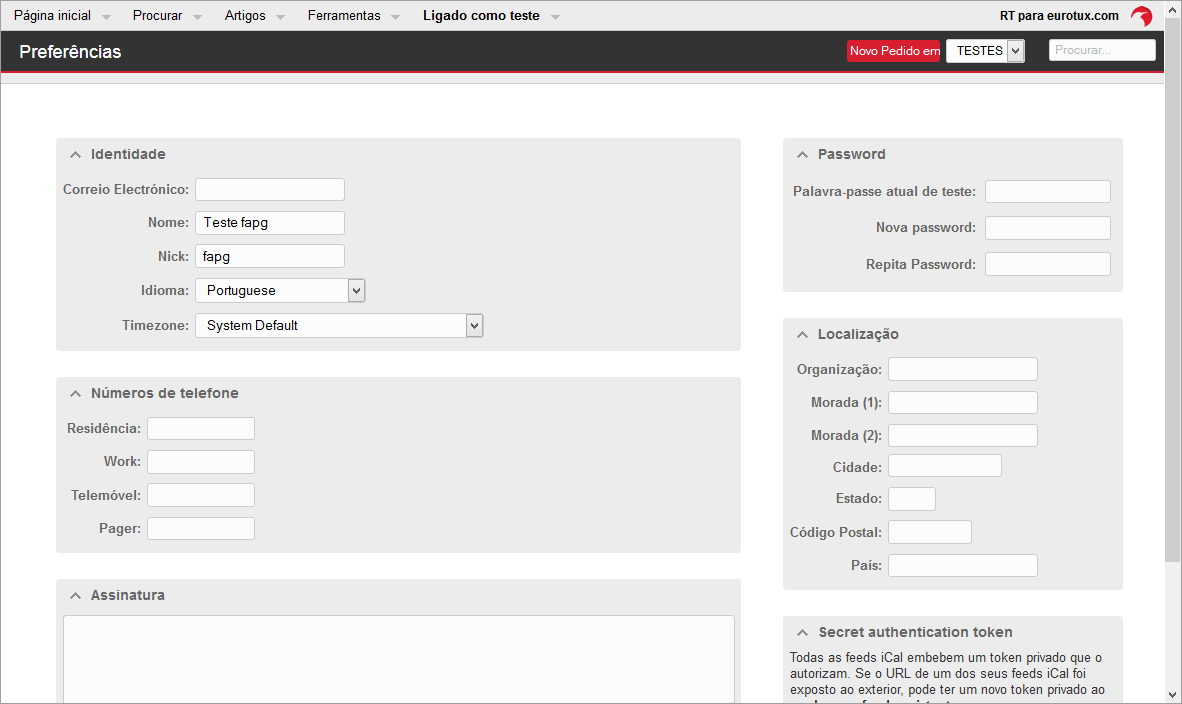
\includegraphics[width=16cm,height=10.5cm]{include/img/rt5-1-PT}
\end{center}
\caption{Alterar preferências.}
\label{fig:boot}
\end{figure}

\section{Sair}
Esta opção encerra a sessão do utilizador, reencaminhando-o para a página inicial.



%\chapter{Página Inicial}
%\section{Descrição}
%
%\chapter{Tickets}
%\section{Descrição}
%\section{Pesquisa Simples}
%\section{Nova Pesquisa}
%
%\chapter{Ferramentas}
%\section{Descrição}
%\section{Artigos}
%\subsection{Visão Geral}
%\subsection{Procura}
%\subsection{topics}
%\section{O Meu Dia}
%\section{Meus Lembretes}
%\section{Offline}
%\section{Aprovação}
%
%\chapter{Ligado como ...}
%\section{Descrição}
%Nesta aba é disponibilizado o acesso às opções de configuração do sistema e a opção para o utilizador efectuar o \textit{logout} do sistema.
%\section{Configurações}
%\subsection{Opções}
%\subsection{Acerca}
%\subsection{Opções de Pesquisa}
%\subsection{Vista inicial RT}
%\subsection{Pesquisa Rápida}
%\subsection{Pesquisas Guardadas}
%\subsubsection*{My Tickets}
%\subsubsection*{Unowned Tickets}
%\subsubsection*{Bookmarked Tickets}
%\section{Sair}
